\documentclass[12pt,a4paper,openright,twoside]{book}
\usepackage[utf8]{inputenc}
\usepackage{disi-thesis}
\usepackage{code-lstlistings}
\usepackage{notes}
\usepackage{shortcuts}
\usepackage{acronym}

\school{\unibo}
\programme{Corso di Laurea Triennale in Ingegneria e Scienze Informatiche}
\title{Tecnologie di Desktop Remoto e il loro Funzionamento}
\author{Matteo Susca}
\date{\today}
\subject{Reti di Telecomunicazioni}
\supervisor{Prof. Franco Callegati}
\session{I}
\academicyear{2023-2024}

% Definition of acronyms
\acrodef{IoT}{Internet of Thing}
\acrodef{vm}[VM]{Virtual Machine}


\mainlinespacing{1.241} % line spacing in mainmatter, comment to default (1)

\begin{document}

\frontmatter\frontispiece

\begin{abstract}	
Max 2000 characters, strict.
\end{abstract}

\begin{dedication} % this is optional
Optional. Max a few lines.
\end{dedication}

%----------------------------------------------------------------------------------------
\tableofcontents   
% \listoffigures     % (optional) comment if empty
% \lstlistoflistings % (optional) comment if empty
%----------------------------------------------------------------------------------------

\mainmatter

%----------------------------------------------------------------------------------------
\chapter{Introduzione}
\label{chap:introduction}

Al giorno d'oggi, è sempre più comune incontrare realtà lavorative che offrono la possibilità di lavorare da remoto. La possibilità di connettersi a un computer aziendale da qualsiasi dispositivo connesso a internet comporta numerosi e innegabili vantaggi, come l'accesso diretto alla rete aziendale, l'utilizzo di hardware specifico per alcune attività senza doverlo trasportare fisicamente, e la flessibilità di lavorare da casa o in mobilità. Tutto questo è reso possibile dalle tecnologie di desktop remoto, che permettono di controllare un computer da un altro dispositivo, ovunque esso si trovi, come se ci si trovasse fisicamente davanti ad esso.

Anche nell'industria videoludica le tecnologie di desktop remoto ricoprono un ruolo importante. Il cloud gaming, ad esempio, è un servizio che permette di giocare a videogiochi in streaming, sfruttando la potenza di calcolo di un server remoto. Il colosso tecnologico NVIDIA, uno dei principali attori in questo settore, ha dimostrato fin dal 2013 con il servizio NVIDIA GRID di essere in grado di offrire un'esperienza di gioco fluida e di alta qualità, grazie all'utilizzo di tecnologie di desktop remoto. Ora il servizio è stato ribattezzato GeForce NOW e offre la possibilità di giocare a numerosi titoli di successo, anche su dispositivi mobili. Anche altre aziende come Google, Microsoft e Amazon stanno investendo in questo settore, con servizi come Google Stadia (attualmente chiuso), Xbox Cloud Gaming e Amazon Luna.

L'assistenza remota è un altro campo in cui le tecnologie di desktop remoto hanno avuto un impatto positivo. I tecnici possono ora accedere al computer di un cliente e risolvere problemi senza doversi recare fisicamente sul posto, riducendo i tempi e i costi di intervento, risultando quindi un vantaggio per entrambe le parti.

Questo lavoro di tesi si propone di analizzare le tecnologie di desktop remoto, partendo dalle loro origini e arrivando alle applicazioni attuali e future. Alla base del desktop remoto e di tecnologie simili vi è il concetto di virtualizzazione del desktop. La virtualizzazione del desktop consiste nella separazione dell'ambiente desktop da un dispositivo fisico attraverso un modello client-server. In questo modello, il desktop virtualizzato viene memorizzato su un server remoto centrale e non sul dispositivo dell'utente. L'utente può quindi accedere a file, applicazioni e dati da qualsiasi dispositivo compatibile, come un PC, un tablet o uno smartphone. % definizione da Desktop Virtualization Frederic P. Miller
Quando invece di un server centrale si utilizza un altro computer come host, si parla specificamente di desktop remoto. Questa tecnologia consente di gestire e controllare da remoto un computer come se ci si trovasse di fronte ad esso fisicamente.

Le tecnologie di desktop remoto hanno subito notevoli cambiamenti nel corso degli anni, evolvendosi in base alle esigenze emergenti e ai progressi tecnologici. Oggi esistono numerosi protocolli tra cui scegliere, ciascuno con le proprie caratteristiche e peculiarità, rispondendo alle diverse esigenze di utilizzo.


%----------------------------------------------------------------------------------------

\chapter{Evoluzione delle Tecnologie di Desktop Remoto}
\label{chap:evolution}
Il voler connettersi da remoto ad un pc è una necessità che si è manifestata fin dai primi anni dell'informatica. Già negli anni '70, insieme al progetto ARPANET, si iniziò a pensare a come poter accedere a terminali remoti tramite una connessione di rete, successivamente implementata con il protocollo Telnet. 
Ovviamente ai giorni nostri, in molti casi, non basta più accedere solamente alla shell di un computer remoto, ma è necessario poter interagire con un'interfaccia grafica. Infatti le esigenze di accesso remoto sono cambiate col tempo e continuano a cambiare. Sono inoltre diverse a seconda del contesto in cui ci si trova: un utente che lavora da casa ha esigenze diverse da un gamer che vuole giocare in mobilità, o da un tecnico che deve risolvere un problema su un computer remoto. Per questo motivo, e per la continua evoluzione delle tecnologie, nel corso degli anni sono stati sviluppati molteplici protocolli e tecnologie con funzionalità e caratteristiche diverse.

\section{Origini prime Tecnologie}
Negli anni '80 esistevano già tecnologie che permettevano di accedere ad un terminale remoto da una macchina locale. Esistevano macchine adibite solamente alla connessione con un terminale remoto; queste macchine erano chiamate "dumb terminal" (terminale stupido) o "thin client". Quest'ultimo termine è ancora utilizzato oggi per indicare un dispositivo che si connette ad un server remoto per eseguire applicazioni e accedere a risorse di rete.
Con l'introduzione e aumento di sistemi operativi con interfaccia grafica, era inevitabile la conseguente evoluzione delle tecnologie di accesso remoto. Fu infatti nel 1984 che fu introdotto, dal Massachusetts Institute of Technology, il X Window System, successore del W Window System.

\section{Analisi e Funzionamento delle Principali Tecnologie di Desktop Remoto} 

\subsection{X Window System}
X Window System, noto anche come X o X11, è un sistema di finestre che consente di eseguire applicazioni grafiche localmente o su computer remoti tramite una architettura client-server. 
Nasce dall'esigenza comune di due progetti del MIT, Athena e il Laboratory for Computer Science, di avere un sistema che permettesse di accedere a risorse grafiche distribuite su una rete di workstation eterogenee, indipendentemente dall'hardware o dal sistema operativo utilizzato \cite{scheifler1986x}. 
Il nome "X" deriva dal suo predecessore, W Window System, sviluppato presso l'Università di Stanford. A differenza di W Window System, X permetteva di gestire applicazioni grafiche su workstation remote, favorendo il concetto di separazione client-server per l'accesso ai display.

La versione attuale di X è la X11, rilasciata nel 1987. Questa versione è stata estesa ulteriormente negli ultimi anni ma il suo funzionamento di base è rimasto invariato e compatibile con le versioni precedenti.

\paragraph{Architettura e Desktop Remoto}
% fonte: https://www.maketecheasier.com/the-x-window-system/ e wikipedia

X è una collezione di software che si posizionano tra l'hardware (o per meglio dire il kernel) e altri software di più alto livello detti X-clients. X si basa su una architettura client-server dove il server è in esecuzione sulla macchina che ospita l'interfaccia grafica e il client è l'applicazione che richiede servizi grafici \cite{scheifler1986x}. Questa terminologia può sembrare controintuitiva in quanto chi non ha familiarità con il sistema X potrebbe pensare che sia invertita. In realtà il tutto deve essere visto dal punto di vista delle applicazioni: queste richiedono servizi grafici e I/O al server X.
I client possono essere locali o remoti. Ogni server X può connettersi a molteplici client.
% immagine architettura X Window System
\begin{figure}
    \centering
    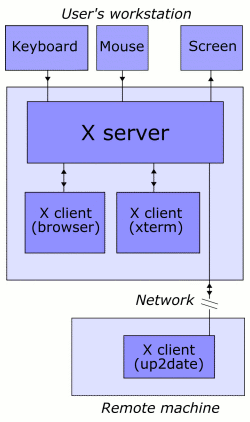
\includegraphics[width=.3\linewidth]{figures/X_client_server_example.png}
    \caption[xarch]{Esempio di architettura client-server di X Window System \footnotemark}
\end{figure}
\footnotetext{Fonte: \url{https://commons.wikimedia.org/wiki/File:X_client_server_example.svg}}

La comunicazione tra server e client avviene in modalità full-duplex, ovvero entrambi possono inviare e ricevere dati contemporaneamente. Lo scambio di messaggi avviene tramite il protocollo TCP/IP, ma spesso vengono utilizzati altri canali comunicativi come Unix domain sockets o memoria condivisa \cite{coopersmith2024x}. Indipendentemente dal canale utilizzato, è necessario che questo sia affidabile e che garantisca l'integrità e l'ordine dei messaggi, in quanto il protocollo X non implementa nativamente meccanismi di ritrasmissione o di ordinamento dei pacchetti.

Quando un client si connette a un server X, avviene una fase di handshake che stabilisce la connessione e verifica l'autenticazione del client. Successivamente, il client può inviare richieste al server, come la creazione di finestre, il disegno di elementi grafici, o la gestione dell'input. Le richieste vengono accumulate in un buffer e inviate in modo asincrono per migliorare l'efficienza della comunicazione. Il server gestisce le richieste di più client contemporaneamente, garantendo l'isolamento tra loro, ma non fornisce alcuna garanzia di ordinamento tra client differenti, a meno che non venga esplicitamente richiesto \cite{coopersmith2024x}.

A differenza di altri protocolli progettati specificamente per il desktop remoto, X è stato sviluppato principalmente per l'esecuzione remota di singole applicazioni grafiche, piuttosto che per la gestione completa di un ambiente desktop (Desktop Environment, DE). Per eseguire un intero DE in remoto, sarebbe necessario ricorrere a software aggiuntivi come X2Go.

Un'altra limitazione del protocollo X è l'assenza di meccanismi di compressione dei dati. Questo significa che i dati grafici vengono trasmessi senza ottimizzazione, il che può causare un utilizzo eccessivo della larghezza di banda e peggiorare le prestazioni su connessioni lente o instabili.

Inoltre, tutta la parte di rendering grafico è demandata alla macchina locale su richiesta del client.

\paragraph{Esempio di utilizzo di X Window System per l'esecuzione remota di applicazioni}

Per comprendere meglio il funzionamento del X Window System in un contesto di desktop remoto, consideriamo un esempio concreto: l'esecuzione dell'applicazione di editing testuale gedit su un server remoto e la sua visualizzazione su un computer locale. Questo può essere realizzato attraverso il X forwarding con ssh, utilizzando il seguente comando:

\begin{lstlisting}[caption={Connessione remota con X forwarding}, label={lst:ssh-x}, language=bash]
ssh -X user@remote_server
\end{lstlisting}

Dopo aver inserito le credenziali e stabilito la connessione, possiamo avviare l'applicazione da linea di comando come avremmo fatto localmente:

\begin{lstlisting}[caption={Esecuzione di gedit su server remoto}, label={lst:gedit}, language=bash]
gedit &
\end{lstlisting}

\paragraph{Funzionamento del protocollo}

Quando viene eseguito il comando \Cref{lst:ssh-x}, il client e il server X avviano una procedura di handshake per stabilire il canale di comunicazione sicuro. Il server X verifica che il client abbia i permessi necessari per connettersi al display locale e, se tutto è corretto, il client e il server negoziano parametri di comunicazione come il byte-ordering, che permette di gestire correttamente i dati tra macchine con architetture diverse \cite{coopersmith2024x}.

Dopo che l'handshake e la negoziazione dei parametri sono stati conclusi, il client remoto \texttt{gedit} invia richieste al server X locale per creare finestre, disegnare interfacce grafiche e gestire l'input dell'utente. Queste richieste vengono trasmesse attraverso il tunnel \texttt{ssh}. Il client chiede inoltre al server X di intercettare gli eventi di input, come la pressione di un tasto o il movimento del mouse, e di inoltrarli al client remoto. Quindi, quando l'utente interagisce con \texttt{gedit} (ad esempio digitando del testo o muovendo il mouse), il server X cattura questi eventi e li inoltra al client remoto tramite il protocollo X11. Il client elabora gli eventi e, se necessario, invia aggiornamenti grafici che vengono visualizzati sul display locale \cite{coopersmith2024x}.

Questo flusso di comunicazione è gestito in modo asincrono, permettendo al server di accumulare richieste in un buffer e processarle in modo efficiente, ottimizzando così l'uso della rete.

\subsection{Citrix XenDesktop}

\subsection{Remote Desktop Protocol}

\subsection{Virtual Network Computing}

\subsection{...}

\chapter{Sviluppi e Applicazioni attuali delle Tecnologie di Desktop Remoto}

\section{Nuove Esigenze e Utilizzi}

\section{Protocolli di Desktop Remoto moderni}

\section{Cloud Gaming e Low-latency Streaming}

\section{...}

\chapter{Prospettive, Sviluppi e Applicazioni futuri del Desktop Remoto}

\section{Desktop as a Service}

\section{Edge Computing}

\section{...}

\chapter{Conclusioni}
\label{chap:conclusions}

%----------------------------------------------------------------------------------------
% BIBLIOGRAPHY
%----------------------------------------------------------------------------------------

\backmatter

\nocite{*} % Remove this as soon as you have the first citation

\bibliographystyle{alpha}
\bibliography{bibliography}

\begin{thebibliography}{9}
    \bibitem{scheifler1986x} 
    R. W. Scheifler and J. Gettys, \textit{The X Window System}, MIT Laboratory for Computer Science, Digital Equipment Corporation, 1986.
    
    \bibitem{coopersmith2024x} 
    A. Coopersmith, \textit{The X New Developer’s Guide: Communication Between Client and Server}, X.org, 2024.
\end{thebibliography}
    

\begin{acknowledgements} % this is optional
Optional. Max 1 page.
\end{acknowledgements}

\end{document}
